\section{Submission to EMDB protocol}
\label{app:exportToEMDB}

Protocol designed to save in a specified folder the three main files required to submit cryo-EM derived electron density maps and derived atomic structures to EMDB (\url{https://deposit-pdbe.wwpdb.org/deposition//}). Although the submission has to be performed online, this protocol tries to help the user to organize their results in different folders according to each particular submission date, project, and so on.

 \begin{itemize}
  \item \scipion menu:
  
    \ttt{Protocols SPA -> Imports} (\ffigure{fig:export_to_EMDB_1} (A))
  
  \item Protocol form parameters (\ffigure{fig:export_to_EMDB_1} (B)):
  
    \begin{figure}[H]
     \centering 
     \captionsetup{width=.7\linewidth} 
     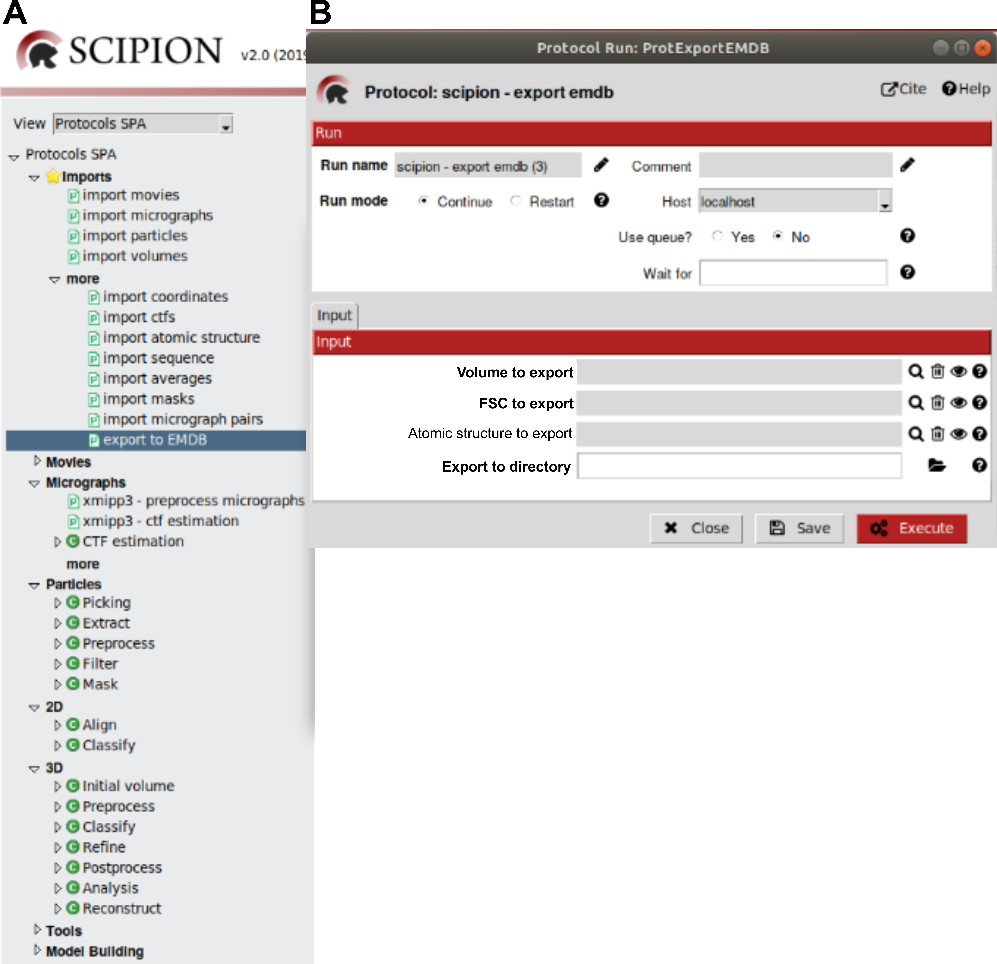
\includegraphics[width=0.90\textwidth]{Images_appendix/Fig156.pdf}
     \caption{Protocol \scommand{export to EMDB}. A: Protocol location in \scipion menu. B: Protocol form.}
     \label{fig:export_to_EMDB_1}
    \end{figure}
    
    \begin{itemize}
     \item \ttt{Input} section

    \begin{itemize}
     \item \ttt{Volume to export}: Param to select the electron density map previously downloaded or generated in \scipion that we would like to submit to EMDB. The map file will be saved with \ttt{.mrc} format.
     \item \ttt{FSC to export}: Param to select the FSC file previously downloaded or generated in \scipion that we would like to submit to EMDB. This file will be saved with \ttt{.xml} format.
     \item \ttt{Atomic structure to export}: Param to select the file of coordinates from the volume-associated atomic structure previously downloaded or generated in \scipion that we would like to submit to EMDB. This file will be saved with \ttt{.cif} format.
     \item \ttt{Export to directory}: Directory specified by the user to save the three above selected files. In order to get appropriate data organization, a name related with the submission is recommended (date, project, number, ...).
    \end{itemize}
   \end{itemize}

  \item Protocol execution:
  
  Adding specific protocol label is recommended in \ttt{Run name} section, at the form top. To add the label, open the protocol form, press the pencil symbol at the right side of \ttt{Run name} box, complete the label in the new opened window, press OK and, finally, close the protocol. This label will be shown in the output summary content (see below). If you want to run again this protocol, do not forget to set to \ttt{Restart} the \ttt{Run mode}.\\
  Press the \ttt{Execute} red button at the form bottom.
  
  The three previously selected files will be saved in the chosen directory after executing the protocol and this can be checked by opening that folder. No additional specific visualization tools have been added to this protocol.

  \item Summary content:
  
   The summary specifies the path to the directory selected to save the three files:\\
   \ttt{Data available at: $path$}
    
\end{itemize}




